
\documentclass{bredelebeamer}
\usepackage{config}
%%%%%%%%%%%%%%%%%%%%%%%%%%%%%%%%%%%%%%%%%%%%%%%%

\title[Teoremas de tipo Bernstein--Doetsch]{
  Teoremas de tipo Bernstein--Doetsch para multifunciones 
  con terminos de error de tipo Takagi--Tabor.
}
% Titre du diaporama

\subtitle{Tesis Doctoral.}
% Sous-titre optionnel

\author [Carlos L. González.]{ 
  Autor: Carlos L. González. (UCV)\\
  Tutor: Dr. Nelson J. Merentes. (UCV) \\
  Co-tutor: Dr. Zsolt Páles. (UNIDEB)
}
% La commande \inst{...} Permet d'afficher l' affiliation de l'intervenant.
% Si il y a plusieurs intervenants: Marcel Dupont\inst{1}, Roger Durand\inst{2}
% Il suffit alors d'ajouter un autre institut sur le modèle ci-dessous.

%\today
% Optionnel. La date, généralement celle du jour de la conférence

\subject{math analysis convexity set-valued maps takagi transformation}
% C'est utilisé dans les métadonnes du PDF


\logo{
  
\includegraphics[scale=0.075]{images/SelloUCV.png}
}

%%%%%%%%%%%%%%%%%%%%%%%%%%%%%%%%%%%%%%%%%%%%%%%%%%%%%%%%%%%%%%%%%%%%%
\begin{document}

\begin{frame}
  \titlepage
\end{frame}

\begin{frame}{Contenido}
  \tableofcontents
  % possibilité d'ajouter l'option [pausesections]
\end{frame}

\section{Antecedentes.}
\subsection{Convexidad.}
\begin{frame}{El concepto de convexidad.}
  \Defi{*}{
    Sea $X$ un espacio normado y $H\subseteq X$ un conjunto no vacío.
    Decimos que el conjunto $H$ es \emph{convexo\footnotemark}, si \alert{para todo}
    par de elementos $x,y \in H$, se tiene que el segmento
    de recta que los une
    \Eq{segment}{
      [x,y] := \{tx + (1-t)y \quad |\quad t\in[0,1]\}
    }
    está, contenido en $H$, i.e., $[x,y]\subseteq H$.
  }
  \begin{figure}
    \centering
    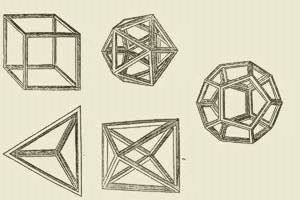
\includegraphics[scale=0.3]{images/davinciplatonic.jpg}
    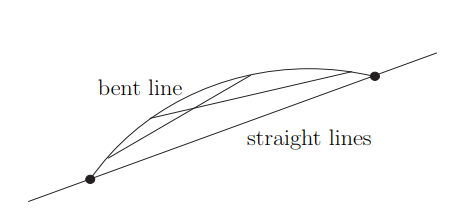
\includegraphics[scale=0.3]{images/convexity_by_archimides.png}
    \caption{Cinco s\'olidos plat\'onicos y la convexidad según Arquímides.}
  \end{figure}
  \footnotetext[1]{
    Hay en un plano ciertas líneas,
    que o bien se encuentran totalmente en el mismo lado 
    de las líneas rectas que unen sus extremidades,
    O no tienen parte de ellos en el otro lado.
    Archimedes of Syracuse (Sicily), ca 287 - ca 212 B.C.
    On the sphere and cylinder \alert{(Incluir referencia)}
  }
\end{frame} % Conjunto convexo
\begin{frame}{Epígrafo de una función.}
  \begin{alertblock}{Notación}
    Sea $X$ un espacio normado, $H\subseteq X$
    un conjunto abierto y convexo de $X$ y 
    $f:H\to \R$ una función.
  \end{alertblock}
  \Defi{*}{
    El \emph{epígrafe} de $f$
    es el conjunto
    \Eq{def_epigraph}{
      \Epi{f} := \{(x,y)\in H\times\R \quad|\quad y \geq f(x)\}
    }
  }
  \Defi{*}{
    Decimos que $f$ es \emph{convexa}
    en $H$ si, $\Epi{f}$ es un conjunto convexo.
  }
  
\end{frame}

\begin{frame}{}
    
  \begin{block}{Observación}
    Sean $x,y\in H$. Note que $(x,f(x)), (y,f(y)) \in\Epi{f}$. Por lo tanto, si 
    $\Epi{f}$ es un conjunto convexo, entonces    
    \Eq{*}{
        t(x,f(x)) &+ (1-t)(y,f(y)) 
          = (tx + (1-t)y, tf(x) + (1-t)f(y)) \in \Epi{f} \quad 
          \forall t\in[0,1], \\
        \mbox{i.e., }& \qquad 
            \fbox{ 
                $f(tx + (1-t)y) \leq tf(x) + (1-t)f(y))  
                    \quad\forall t\in[0,1],$ 
            }
    }
  \end{block}
  \Prp{*}{
    $f$ es \emph{convexa} en $H$ sii, para todo $x,y\in H$ 
    se tiene que 
    \Eq{cvx}{
      f(tx + (1-t)y) \leq tf(x) + (1-t)f(y), \quad t\in[0,1].
    }
  }
  \Defi{*}{
    Diremos que $f$ es \emph{cóncava} en $H$ si para todo $x,y\in H,$ 
    se tiene que 
    \Eq{cvx}{
        tf(x) + (1-t)f(y) \leq f(tx + (1-t)y), \quad t\in[0,1].
    }
  }
\end{frame} % Epgirafo de una función y definicion de funcion convexa
\begin{frame}{Función midconvexa y $\Q$-convexidad.}
  \Defi{*}{
    Diremos que la función $f$ es \emph{midconvexa}, si la 
    ecuación \eq{cvx} se cumple para $t=\frac12.$ Es
    decir, si para todo $x,y\in H$ se tiene que 
    \Eq{midcvx}{
        f\bigg(\frac{x+y}{2}\bigg)\leq\frac{f(x) + f(y)}2.
    }
  }
  \Defi{*}{
    Diremos que la función $f$ es \emph{$\Q$-convexa}, 
    si para todo $x,y\in H$ se tiene que 
    \Eq{qcvx}{
        f(tx + (1-t)y) \leq tf(x) + (1-t)f(y), \quad t\in[0,1]\cap\Q.
    }
  }
\end{frame}

\begin{frame}{Algunas observaciones.}
    \begin{exampleblock}{Observación}
        La desigualdad 
        \Eq{*}{
            f\bigg(\frac{x+y}{2}\bigg)\leq\frac{f(x) + f(y)}2.
        }
        implica que para todo $n\in\NN, x_1,x_2, \ldots, x_n\in H$
        \Eq{*}{
            f\bigg(\frac{x_1 + x_2 + \cdots + x_n}{n}\bigg)\leq\frac{f(x_1) + f(x_2) + \cdots + f(x_n)}n.
        }
        y a su vez, esto último implica que si $p,q\in\NN$, $q\neq0$, entonces 
        \Eq{*}{
            f\bigg(\frac{px + (q-p)y}{q}\bigg)\leq\frac{pf(x) + (q-p)f(y)}q.
        }
    \end{exampleblock}
    \Thm{*}{
        $f$ es midconvexa en $H$, si y sólo si, $f$ es $\Q$-convexa en $H$.
    }{Referencia}
\end{frame}

\subsection{El teorema de Bernstein--Doetsch.}
\begin{frame}{Teoremas de tipo Bernstein--Doetsch.}
    \Thm{*}{
        Toda función midconvexa y continua en $H$ es convexa.
    }{\cite{Kuc85}, Theorem 5.3.5.}
    \Thm{*}{
        Toda función midconvexa y localmente acotada superior
        en un punto, es convexa.
    }{\cite{Kuc85}, Theorem 6.4.2, \cite{BerDoe15}}
    \startchronology[startyear=1984,stopyear=2018,color=blue!50!white,arrow=false,dateselevation=5pt,height=5pt]
	
	\chronoevent[date=false,markdepth=70pt]{2017}{\tiny{\cite{GilGonNikPal15}}}
	\chronoevent[date=false,markdepth=60pt]{2014}{\tiny{\cite{GonNikPalRoa14}}}
	\chronoevent[date=false,markdepth=40pt]{2013}{\tiny{\cite{LeiMerNikSan13}}}
	\chronoevent[date=false,markdepth=25pt,ifcolorbox=false]{2012}{\tiny{\cite{MakPal12a}}}
	\chronoevent[date=false,markdepth=32pt,mark=false,ifcolorbox=false]{2012}{\tiny{\cite{Mur12DM}}}
	\chronoevent[date=false,markdepth=60pt]{2011}{\tiny{\cite{AzoGimNikSan11}}}
	\chronoevent[date=false,markdepth=68pt,mark=false,ifcolorbox=false]{2011}{\tiny{\cite{Haz11}}}
	\chronoevent[date=false,markdepth=73pt,mark=false,ifcolorbox=false]{2011}{\tiny{\cite{GilTro11}}}
	
	\chronoevent[date=false,ifcolorbox=false,markdepth=40pt]{2010}{\tiny{\cite{HazBur10}}}
	\chronoevent[date=false,ifcolorbox=false,markdepth=45pt]{2010}{\tiny{\cite{Haz10}}}
	\chronoevent[date=false,ifcolorbox=false]{2009}{\tiny{\cite{TabTab09a}}}
	\chronoevent[date=false,markdepth=18pt,mark=false,ifcolorbox=false]{2009}{\tiny{\cite{BurHazJuh09}}}
	\chronoevent[date=false,markdepth=25pt,mark=false,ifcolorbox=false]{2009}{\tiny{\cite{Haz09a}}}
	\chronoevent[date=false]{2005}{\tiny{\cite{HazPal05}}}
	\chronoevent[date=false,markdepth=40pt]{2004}{\tiny{\cite{HazPal04}}}
	\chronoevent[date=false,markdepth=50pt,mark=false]{2004}{\tiny{\cite{GilNikPal04}}}
	\chronoevent[date=false,markdepth=22pt,ifcolorbox=false]{2003}{\tiny{\cite{Nik03}}}
	\chronoevent[date=false,markdepth=30pt]{2001}{\tiny{\cite{Nik01}}}
	\chronoevent[date=false,markdepth=40pt,mark=false]{2001}{\tiny{\cite{NikPal01}}}
	\chronoevent[date=false,ifcolorbox=false]{2000}{\tiny{\cite{Pal00b}}}
	
	\chronoevent[date=false,markdepth=30pt]{1999}{\tiny{\cite{ChadMir99JST}}}
	\chronoevent[date=false]{1993}{\tiny{\cite{NgNik93}}}
	\chronoevent[date=false,markdepth=40pt]{1991}{\tiny{\cite{KomKuc91b}}}
	
	\chronoevent[date=false,markdepth=20pt,mark=false]{1989}{\tiny{\cite{Nik89}}}
	\chronoevent[date=false]{1989}{\tiny{[KomKuc89]\nocite{KomKuc89b}}}
	\chronoevent[date=false,markdepth=40pt]{1987}{\tiny{\cite{Nik87a}}}
	\chronoevent[date=false,ifcolorbox=false,markdepth=50pt,mark=false]{1987}{\tiny{\cite{Nik87c}}}
	\chronoevent[date=false,ifcolorbox=false]{1986}{\tiny{\cite{Nik86}}}
	\chronoevent[date=false,ifcolorbox=false]{1984}{\tiny{\cite{Tru84}}}
	
\stopchronology
\end{frame} % Una equivalencia para la convexidad de f
\subsection{Convexidad aproximada.}
\begin{frame}{Función de Takagi}
	\Defi{*}{
    	La función $T:\R\to[0,1]$ definida mediante la fórmula 
    	\Eq{Tak}{
    	    T(t) = \sum_{n=0}^{\infty}\frac1{2^n}\dist(2^nt,\Z),\qquad(t\in\R),
    	}
    	se conoce como la función de \emph{Takagi}.
	}
	\begin{block}{Observación.}
    	\Eq{*}{
    	    T(t) = \limit_{n\to\infty} T_n(t),\quad t\in\R
    	}
    	donde
    	\Eq{*}{
    	    T_n(t) = T_{n-1}(t) +\frac1{2^n}\dist(2^nt,\Z), \quad n\in\NN,t\in\R,
    	}
    	y además $T_0(t) = \dist(t,\Z).$
	\end{block}
\end{frame} % funcion de takagi.
\begin{frame}{Convexidad aproximada.}
    Sean $\varepsilon, \delta \geq 0$, 
    $f:H\to \R$ y $\alpha:\R^+\to\R^+$, una función no-decreciente.
    \DefiOp{*}{
        \begin{itemize}
            \item $f$ es \emph{$\varepsilon$-midconvexa} si para todo $x,y\in H$ 
            	\Eq{*}{
            	    f\bigg(\cmcvx{x}{y}\bigg)\leq \cmcvx{f(x)}{f(y)} +\varepsilon.
            	}
            \item $f$ es \emph{$(\delta,\varepsilon)$-midconvexa} en $H,$ si para todo $x,y \in H$
            	\Eq{*}{
            	    f\bigg(\cmcvx{x}{y}\bigg)\leq \cmcvx{f(x)}{f(y)}+\delta\|x-y\|+\varepsilon
            	}
            \item $f$ es \emph{$\alpha(\cdot)$-midconvexa} en $H,$ si para todo $x,y \in H$
        		\Eq{e-Cvx}{
        			f\bigg(\frac{x+y}2\bigg) \leq \frac{f(x)+f(y)}2 + \alpha(\|x-y\|).
        		}
        \end{itemize}
	}{\cite{HyeUla52}, \cite{HazPal04}, \cite{TabTab09b}}
\end{frame} % e-convexity.
\begin{frame}{$(\varepsilon,\delta)$-Convexidad}
	\Thm{*}{
    	\label{TNgNik}
    	Si $f:H\to\R$ es una función localmente acotada superior en un punto de $H$, y
    	$\varepsilon$-midconvexa entonces, $f$ es $2\varepsilon$-convexa, i.e,
    	para todo $x,y\in H$ y para todo $t\in[0,1]$
    	\Eq{*}{
    	    f(tx+(1-t)y)\leq tf(x)+(1-t)f(y)+2\varepsilon.
    	}
	}{\cite{NgNik93,Lac99}} 
	\Thm{*}{
	    \label{THazPal3}
    	Sean $\delta$ y $\varepsilon$ dos números no negativos. Si $f:H\to\R$ es una función
    	$(\delta,\varepsilon)$-midconvexa acotada superiormente en un punto de $H$ entonces,
    	para todo $x,y\in H$ y para todo $t\in(0,1)$
    	\Eq{HazPal33}{
    	    f(tx+(1-t)y) \leq tf(x)+(1-t)f(y)+2\delta T(t)\|x-y\|+2\varepsilon
    	}
	    donde $T$ es la función de Takagi definida en \eq{Tak}.
	}{\cite{HazPal04}, Teorema 4}
\end{frame}
 % e,delta-convexity.
\begin{frame}
	\Thm{*}{
    	La función de Takagi es $\big(\frac12,0\big)$-midconvexa, i.e.,
    	\Eq{*}{
    	    T\bigg(\cmcvx{x}{y}\bigg)\leq \cmcvx{T(x)}{T(y)}+\Big|\frac{x-y}2\Big|,
    	}
    	para todo $x,y\in\R$.
    	}{\cite{Bor08}}
	\begin{exampleblock}{Observación}
    	Supongamos que el teorema anterior sigue siendo válido si se reemplaza
    	$T$ por una función $\phi$ arbitraria.
    	Aplicando el Teorema HP a la función de Takagi, obtenemos
    	que para todo $x,y\in\R$ y todo $\lambda\in[0,1]$
    	\Eq{*}{
    	    T(\lambda x+(1-\lambda)y) \leq \lambda T(x)+(1-\lambda)T(y)+\phi(\lambda )|x-y|.
    	}
    	En particular, para $x=1$ y $y=0$ la ecuación anterior se convierte en
    	\Eq{*}{
    	    T(\lambda) \leq \phi(\lambda).
    	}
    \end{exampleblock}
\end{frame} % takagi function and e,delta-convexity.
\begin{frame}{J. Mako, Z. Pales, J. Tabor, J.Tabor}
	\Thm{*}{
		Sea $D\subseteq \R$ un subconjunto abierto y convexo de la recta real.
		Si $f:D\to\R$ es una función localmente acotada superior en un punto y 
		$\alpha$-midconvexa en $D$, entonces, para todo $x,y\in D$ y para todo
		$t\in[0,1]$ 
		\Eq{*}{
		    f(tx + (1-t)y)\leq 
		        tf(x) + (1-t)f(y) + 
		        \sum_{n=0}^{\infty}\frac{1}{2^n}\alpha(2\dist_\Z(2^nt)\|x-y\|).
		}
% 		donde 
% 		\Eq{*}{
%     		\T_\alpha(t,u)=\sum_{n=0}^{\infty}\frac{1}{2^n}\alpha(2\dist_\Z(2^nt)u),\quad
%     		t\in[0,1], u\in D-D.
% 		}
	}{\cite{HazPal04,MakPal10b}}
	
	\Thm{*}{
		Sea $D\subseteq \R$ un subconjunto abierto y convexo de la recta real.
		Si $\sum_{n=0}^\infty\alpha(2^{-n})<\infty$ y
		$f:D\to\R$ es una función localmente acotada superior en un punto y 
		$\alpha$-midconvexa en $D$, entonces, para todo $x,y\in D$ y para todo
		$t\in[0,1]$ 
		\Eq{*}{
    		f(tx + (1-t)y)\leq 
    		    tf(x) + (1-t)f(y) + 
    		    \sum_{n=0}^{\infty}2\dist_\Z(2^nt)\alpha\Bigg(\frac{\|x-y\|}{2^{n+1}}\Bigg).
		}
% 		donde 
% 		$$
% 		\MS_\alpha(t,u)=\sum_{n=0}^{\infty}2\dist_\Z(2^nt)\alpha\Big(\frac{u}{2^{n+1}}\Big),\quad
% 		t\in[0,1], u\in D-D.
% 		$$
	}{\cite{TabTab09b}}
\end{frame} % takagi function and e,delta-convexity.
\subsection{Convexidad fuerte.}
\begin{frame}{Convexidad fuerte}
    \DefiOp{*}{
    	Sea $c>0$. Se dice que una función $f:D\to\R$ 
    	es fuertemente midconvexa con módulo $c$, si 	
    	para todo $x,y\in D$ y $t\in[0,1]$
    	\Eq{strgMidPol}{
    	    f\bigg(\frac{x+y}{2}\bigg)\leq \frac{f(x)+f(y)}2-\frac{c}4\|x-y\|^2,
    	}
	}{\cite{Pol66}}
	\Thm{*}{
    	Sea $c>0$. Si $f:D\to\R$ es una función fuertemente midconvexa 
    	con módulo $c$ y acotada superiormente en un subconjunto de $D$ 
    	con interior no vacío, entonces, $f$ es una función continua
    	y además fuertemente convexa con módulo $c$, i.e.,
    	\Eq{strgPol}{
    	    f(tx+(1-t)y)\leq tf(x)+(1-t)f(y)-ct(1-t)\|x-y\|^2,
    	}
	    para todo $x,y\in D,$ $t\in[0,1]$.
	}{\cite{AzoGimNikSan11}}
\end{frame}
\begin{frame}{Multifunciones.}
  Sean $X$ y $Y$ espacios topol\'ogicos lineales y sea $D\subseteq X$
  un subconjunto abierto y convexo. Denotemos por $\P_0(Y)$ a la clase
  de subconjuntos no-vac\'ios de $Y$.
  \Defi{*}{
    Una multifunci\'on $F:D\to\P_0(Y)$ es midconvexa en $D,$ si para todo
    $x,y\in D$ se satisface 
    \Eq{*}{
      \cmcvx{F(x)}{F(y)} \subseteq F\bigg(\cmcvx{x}{y}\bigg).
    }
  }
  \Defi{*}{
    Una multifunci\'on $F:D\to\P_0(Y)$ es midc\'oncava en $D,$ si para todo
    $x,y\in D$ se satisface 
    \Eq{*}{
      F\Xbigg(\cmcvx{x}{y}\bigg)\subseteq\cmcvx{F(x)}{F(y)}.
    }
  }
\end{frame} % multifunciones

\section{Referencias}
\begin{frame}[allowframebreaks]
  \frametitle{Referencias}
  \scriptsize{\bibliographystyle{amsalpha}}%amsalpha
  \bibliography{publ,funcequ}
  \beamertemplatearticlebibitems
\end{frame}

\end{document}
